\documentclass[12pt,a4paper]{report}
\usepackage[english]{babel}
\usepackage[left=2.5cm,right=2.5cm,top=2cm,bottom=1.5cm]{geometry}
\usepackage[T1]{fontenc}
\usepackage{graphicx}
\usepackage{hyperref}
\usepackage{multirow}
\usepackage[table]{xcolor}

% Select Arial font for the whole document
\usepackage{helvet}
\renewcommand{\familydefault}{\sfdefault}


\usepackage[a4paper, includehead,
textwidth=16cm, textheight=23cm,
headheight=2.7cm,
%showframe,
]{geometry}


\usepackage{fancyhdr}

% AD and RD entries
\usepackage{enumerate}
\usepackage[shortlabels]{enumitem}

\newenvironment{ADlist}
               {\begin{enumerate}[start=1,label={AD\arabic*}]}  % \bfseries
               {\end{enumerate}}               
\newenvironment{RDlist}
               {\begin{enumerate}[start=1,label={RD\arabic*}]}  % \bfseries
               {\end{enumerate}}
\newcommand{\ARDitem}[2]{\item \label{#1} {#2}}
\newcommand{\citedoc}[1]{[\ref{#1}]}


% List of requirements
\usepackage{tocloft}
\newcommand{\listreqname}{List of Requirements:}
\newlistof{req}{toreq}{\listreqname}
\newcommand{\req}[2]{%
\refstepcounter{req}
\par\vspace{0.2cm}\noindent\textbf{\esoreqprefix{}\thereq:} #2 \label{#1}\vspace{0.2cm}
\addcontentsline{toreq}{req}
{\protect \textbf{\esoreqprefix{}\numberline{\thereq}}#2}\par}
\newcommand{\citereq}[1]{\textbf{\esoreqprefix{}\ref{#1}}}


% List of questions
\newcommand{\listquestionname}{List of Questions:}
\newlistof{question}{toquestion}{\listquestionname}
\newcommand{\question}[2]{%
\refstepcounter{question}
\par\vspace{0.2cm}\noindent\textbf{Q\thequestion:} #2 \label{#1}\vspace{0.2cm}
\addcontentsline{toquestion}{question}
{\protect \textbf{Q\numberline{\thequestion}}#2}\par}
\newcommand{\citequestion}[1]{\textbf{Q\ref{#1}}}


% Title page
\newcommand{\esotitlepage}[1]{
\thispagestyle{empty}
\begingroup
%\setlength{\tabcolsep}{10pt}       % Default value: 6pt
\renewcommand{\arraystretch}{1.5}   % Default value: 1
\begin{center}
  \begin{tabular}{|p{0.3\textwidth}|p{0.7\textwidth}|}
    \hline
        {\bf \small Document title:}          & {\bf \esodoctitle{}}         \\[0.8cm] \hline
        {\bf \small Document number:}         &      \esodocnumber{}         \\[0.8cm] \hline
        {\bf \small Document verision:}       &      \esodocversion{}        \\[0.8cm] \hline
        {\bf \small Document type:}           &      \esodoctype{}           \\[0.8cm] \hline
        {\bf \small Document status:}         &      \esodocstatus{}         \\[0.8cm] \hline
        {\bf \small Releasing organization:}  &      \esodocorganization{}   \\[0.8cm] \hline
        {\bf \small Released on:}             &      \esodocreleasedate      \\[0.8cm] \hline
        {\bf \small Document classification:} &      \esodocclassification{} \\[0.8cm] \hline
  \end{tabular}
\end{center}

\vspace{3cm}

#1

\endgroup

\newpage

}



% Running header
\newcommand{\esoheader}{
\pagestyle{fancy}
\fancyhead{} % clear all header fields
\fancyfoot{} % clear all footer fields
\renewcommand{\headruleskip}{1.2mm}
\fancyhead[L]{
  \begin{tabular}{m{0.12\headwidth}p{0.34\headwidth}}
    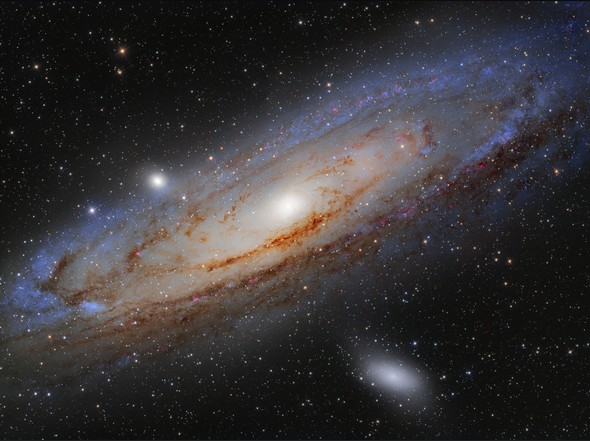
\includegraphics[width=2.2cm]{media/header_logo.jpg}  &  {\small \esodoctitle{}}\\
  \end{tabular}
}
\fancyhead[R]{
    \footnotesize
    \begin{tabular}{|p{0.2\headwidth}|p{0.21\headwidth}|}
      \hline
        {Document number:}         &      \esodocnumber{}     \\\hline
        {Document verision:}       &      \esodocversion{}    \\\hline
        {Document status:}         &      \esodocstatus{}     \\\hline
        {Released on:}             &      \esodocreleasedate  \\\hline
        {Page:}                    &      \thepage{} of \pageref{LastPage} \\\hline
    \end{tabular}
}
}



\begin{document}

\begin{center}
  \begin{tabular}{ l l }
    \hline
        {\bf Document title:}          & {\bf CUBES design}                       \\ \hline
        {\bf Document number:}         & CUBES-123-456-789                        \\ \hline
        {\bf Document verision:}       & 0.1                                      \\ \hline
        {\bf Document type:}           & XXX                                      \\ \hline
        {\bf Document status:}         & Draft                                    \\ \hline
        {\bf Releasing organization:}  & CUBES Consortium                         \\ \hline
        {\bf Released on:}             & 2023-01-01                               \\ \hline
        \multirow{2}{*}{\bf Document classification:} & CUBES Consortium Internal \\
                                       & [Confidential for non-CUBES staff]       \\ \hline
  \end{tabular}
\end{center}

\vfill

\begin{center}
\begin{tabular}{ l l l }
    \hline
    \textbf{Prepared by:} &  Giorgio Calderone (CUBES SSE) & \begin{minipage}[c]{0.1\textwidth}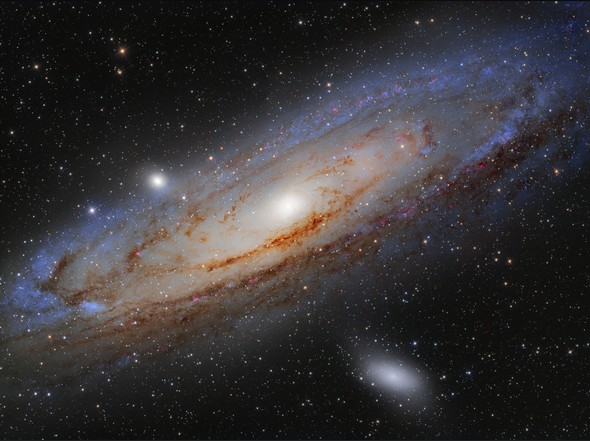
\includegraphics[width=0.3\textwidth]{media/m31.jpg} \end{minipage} \\
    \textbf{Apporved by:} &  Roberto Cirami (CUBES PM)     & \begin{minipage}[c]{0.1\textwidth}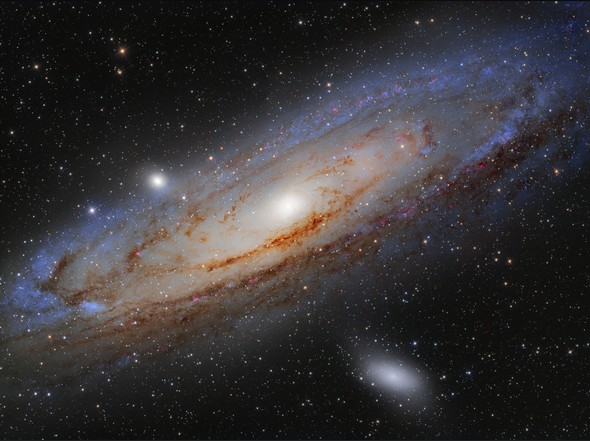
\includegraphics[width=0.3\textwidth]{media/m31.jpg} \end{minipage} \\
    \textbf{Released by:} &  Roberto Cirami (CUBES PM)     & \begin{minipage}[c]{0.1\textwidth}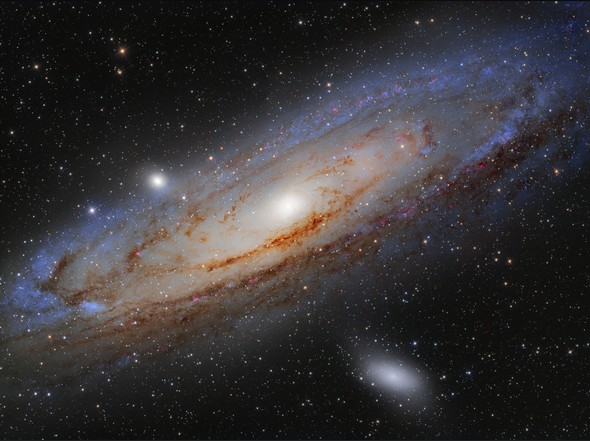
\includegraphics[width=0.3\textwidth]{media/m31.jpg} \end{minipage} \\
    \hline
    \end{tabular}
\end{center}


\newpage


{\Large \bf Authors}
\medskip

\begin{tabular}{ |p{6cm}|p{8cm}| }
  \hline
      {\bf Name} & {\bf Affiliation}\\
      \hline
      Giorgio Calderone & INAF-OATs\\
      \hline
\end{tabular}

\bigskip

{\Large \bf Change Record from previous Version}
\medskip

\begin{tabular}{ |p{4cm}|p{10cm}| }
  \hline
      {\bf Affected Section(s)} & {\bf Changes / Reason / Remarks}\\
      \hline
       & \\
      \hline
\end{tabular}


\newpage

\tableofcontents

\newpage

\chapter{Introduction}

Lorem ipsum dolor sit amet, consectetur adipiscing elit, sed do eiusmod tempor incididunt ut labore et dolore magna aliqua. Ut enim ad minim veniam, quis nostrud exercitation ullamco laboris nisi ut aliquip ex ea commodo consequat. Duis aute irure dolor in reprehenderit in voluptate velit esse cillum dolore eu fugiat nulla pariatur. Excepteur sint occaecat cupidatat non proident, sunt in culpa qui officia deserunt mollit anim id est laborum.


\begin{equation}
  \label{eq:eq}
  E = mc^2
\end{equation}

\begin{enumerate}
\item {\bf bold};
\item {\it italic};
\item {\tt teletype};
\item normal\footnote{Footnote test};
\item {\tiny tiny};
\item {\small small};
\item {\large large};
\item {\Large Large}.
\end{enumerate}


\chapter{Related documents}

The following documents, of the exact version shown, form part of this document to the extent specified herein. In the event of conflict between the documents referenced herein and the content of this document, the content of this document shall be considered as superseding.  AD references shall be specific about which part of the target document is the subject of the reference.

\section{Applicable documents}
\begin{ADlist}
  \ARDitem{AD:ISURS}{CUBES Instrument Software User Requirement Specifications;\\CUBES-SWR-SPE-004, Version 1;}
  \ARDitem{AD:ESO-379353}{Common Requirements for VLT Instruments;\\ESO-379353, Version 3}
  \ARDitem{AD:ESO-351071}{ICS Software Specification;\\ESO-351071, Version 1}
\end{ADlist}


\section{Reference documents}
\begin{RDlist}
  \ARDitem{RD:ESO-351097}{VLT-ELT Gateway Software Design Description;\\ESO-351097, Version 2}
  \ARDitem{RD:ESO-363357}{ELT ICS Framework - Online Data Processing - User Manual;\\ESO-363357, Version 2}
  \ARDitem{RD:ESO-363358}{ELT ICS Framework - Sequencer - User Manual;\\ESO-363358, Version 1}
\end{RDlist}



\chapter{Main matter}

\section{Requirements}
Lorem ipsum dolor sit amet, consectetur adipiscing elit, sed do eiusmod tempor incididunt ut labore et dolore magna aliqua. Ut enim ad minim veniam, quis nostrud exercitation ullamco laboris nisi ut aliquip ex ea commodo consequat. Duis aute irure dolor in reprehenderit in voluptate velit esse cillum dolore eu fugiat nulla pariatur. Excepteur sint occaecat cupidatat non proident, sunt in culpa qui officia deserunt mollit anim id est laborum.
\req{req:must_work}{CUBES must work.}

Lorem ipsum dolor sit amet, consectetur adipiscing elit, sed do eiusmod tempor incididunt ut labore et dolore magna aliqua. Ut enim ad minim veniam, quis nostrud exercitation ullamco laboris nisi ut aliquip ex ea commodo consequat. Duis aute irure dolor in reprehenderit in voluptate velit esse cillum dolore eu fugiat nulla pariatur. Excepteur sint occaecat cupidatat non proident, sunt in culpa qui officia deserunt mollit anim id est laborum.

\req{req:must_notbreak}{CUBES must not break.}

\section{Questions}

Lorem ipsum dolor sit amet, consectetur adipiscing elit, sed do eiusmod tempor incididunt ut labore et dolore magna aliqua. Ut enim ad minim veniam, quis nostrud exercitation ullamco laboris nisi ut aliquip ex ea commodo consequat. Duis aute irure dolor in reprehenderit in voluptate velit esse cillum dolore eu fugiat nulla pariatur. Excepteur sint occaecat cupidatat non proident, sunt in culpa qui officia deserunt mollit anim id est laborum.
\question{q:how_to}{How to make a coffee?}

Lorem ipsum dolor sit amet, consectetur adipiscing elit, sed do eiusmod tempor incididunt ut labore et dolore magna aliqua. Ut enim ad minim veniam, quis nostrud exercitation ullamco laboris nisi ut aliquip ex ea commodo consequat. Duis aute irure dolor in reprehenderit in voluptate velit esse cillum dolore eu fugiat nulla pariatur. Excepteur sint occaecat cupidatat non proident, sunt in culpa qui officia deserunt mollit anim id est laborum.

\question{q:when_to}{When to make a coffee?}

\section{Figures and tables}

\begin{figure}[hbtp!]
  \centering
  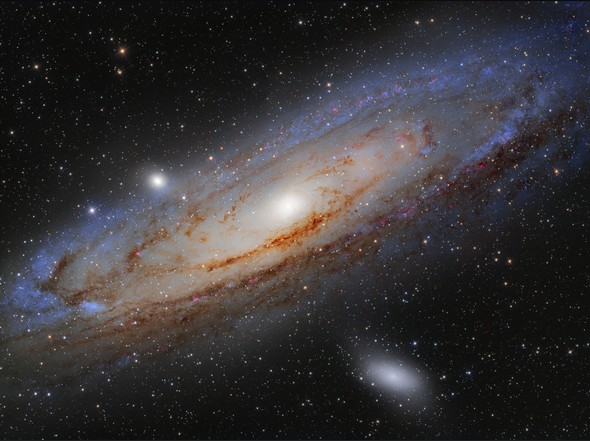
\includegraphics[width=0.5\textwidth]{media/m31}
  \caption{Andromeda galaxy}
    \label{fig:m31}
\end{figure}


\begin{table}[hbtp!]
  \centering
  \begin{tabular}{ |l|l|l| }
    \hline
    \rowcolor{lightgray} \multicolumn{3}{|c|}{Country List} \\
    \hline
    Country Name or Area Name& ISO ALPHA 2 Code &ISO ALPHA 3 \\
    \hline
    Afghanistan & AF &AFG \\
    \rowcolor{gray}
    Aland Islands & AX & ALA \\
    Albania   &AL & ALB \\
    Algeria  &DZ & DZA \\
    American Samoa & AS & ASM \\
    Andorra & AD & \cellcolor[HTML]{AA0044} AND    \\
    Angola & AO & AGO \\
    \hline
  \end{tabular}
  \caption{Table to test captions and labels.}
  \label{tab:test}
\end{table}


\section{References}
\begin{itemize}
\item \ref{AD:ISURS}, \ref{RD:ESO-363358};
\item \citereq{req:must_work}, \citereq{req:must_notbreak}
\item \citequestion{q:how_to}, \citequestion{q:when_to};
\item Tab.~\ref{tab:test}, Fig.~\ref{fig:m31}, Eq.~\ref{eq:eq};
\end{itemize}


\newpage

\listofreq
\listofquestion

\end{document}

